\documentclass[12pt]{book}
\usepackage{cdt/cdtBusiness}
\usepackage{requerimientos}
\usepackage{graphicx}
\usepackage{paear}
\usepackage{subfigure}
\usepackage{cite}
\usepackage{float}
\usepackage[spanish]{babel}
\usepackage{pdfpages}
\usepackage{lscape}

%%%%%%%%%%%%%%%%%%%%%%%%%%%%%%%%%%%%%%%%%%%%%%%%%%%%%%%%%%%%%%%%
% Datos del proyecto

\organizacion[]{Escuela Superior de Cómputo}
\autor[]{Instituto Politécnico Nacional}
\sistema[]{Asistente Móvil para el Seguimiento de Tratamientos Médicos (Rem-Pills)}
\proyecto[]{}
\documento{}{Documento Técnico Etapa 2}%{\RELEASE{1.0}}%{\DRAFT{\today}} 

\entregable{}{\Large{Asistente Móvil para el Seguimiento de Tratamientos Médicos (Rem-Pills)}}

% Descomentar y establecer la fecha cuando se desee congelar la fecha del documento.
%\fecha{12 de Abril de 2013}

%%%%%%%%%%%%%%%%%%%%%%%%%%%%%%%%%%%%%%%%%%%%%%%%%%%%%%%%%%%%%%%%
% Datos para revisión
%\elaboro[Alumnos de la Licenciatura en Ingeniería en Sistemas Computacionales IPN - ESCOM]{Cesar Raúl Avila Padilla\vspace{0.4cm} Ivo Sebastián Sam Álvarez-Tostado\vspace{0.4cm}} % Responsable del contenido (IPN) Lic. Ulises Vélez Saldaña
%\superviso[Alumnos de la Licenciatura en Ingeniería en Sistemas Computacionales IPN - ESCOM]{Cesar Raúl Avila Padilla\vspace{0.4cm} Ivo Sebastián Sam Álvarez-Tostado\vspace{0.4cm}}
%\aprobo[Directores del Trabajo Terminal 2017-A108]{M. en C. Ulises Velez Saldaña\\ M. en C. José David Ortega Pacheco} % Responsable Técnico (Contraparte)

%\title{\varProyecto}
%\subtitle{\varCveDocumento--\varDocumento}


%%%%%%%%%%%%%%%%%%%%%%%%%%%%%%%%%%%%%%%%%%%%%%%%%%%%%%%%%%%%%%%%
% Documentos relacionados con el documento actual

% TODO: Escriba los documentos en los que está basado este documento.

%%%%%%%%%%%%%%%%%%%%%%%%%%%%%%%%%%%%%%%%%%%%%%%%%%%%%%%%%%%%%%%%
% Elementos contenidos en el documento

% TODO: Al finalizar el análisis resuma aquí todos los elementos del componente: RN, CU, IU, MSG.
%\elemRefs{
%
%	%Glosario de términos
%   \elemItem{Glosario de términos}{1.0}{Descripción de los terminos técnicos y de negocio utilizados}
%%---------------------------------------------------------------------------------------------------------------------------------------
%
%	%Modelo de información
%   \elemItem{Modelo Registro de escuelas}{1.0}{Descripción del modelo de información del Registro de escuelas}
%
%}

%%%%%%%%%%%%%%%%%%%%%%%%%%%%%%%%%%%%%%%%%%%%%%%%%%%%%%%%%%%%%%%%
\begin{document}
\renewcommand{\listtablename}{Índice de tablas}
\renewcommand{\tablename}{Tabla} 

%=========================================================
% Portada
\ThisLRCornerWallPaper{1}{cdt/theme/agua.png}
\thispagestyle{empty}


\includepdf[pages=1-1]{portadaTT2.pdf}

\includepdf[pages=1-1]{HojaPresentacion.pdf}

\includepdf[pages=1-1]{cartaResponsivaTT_20191.pdf}
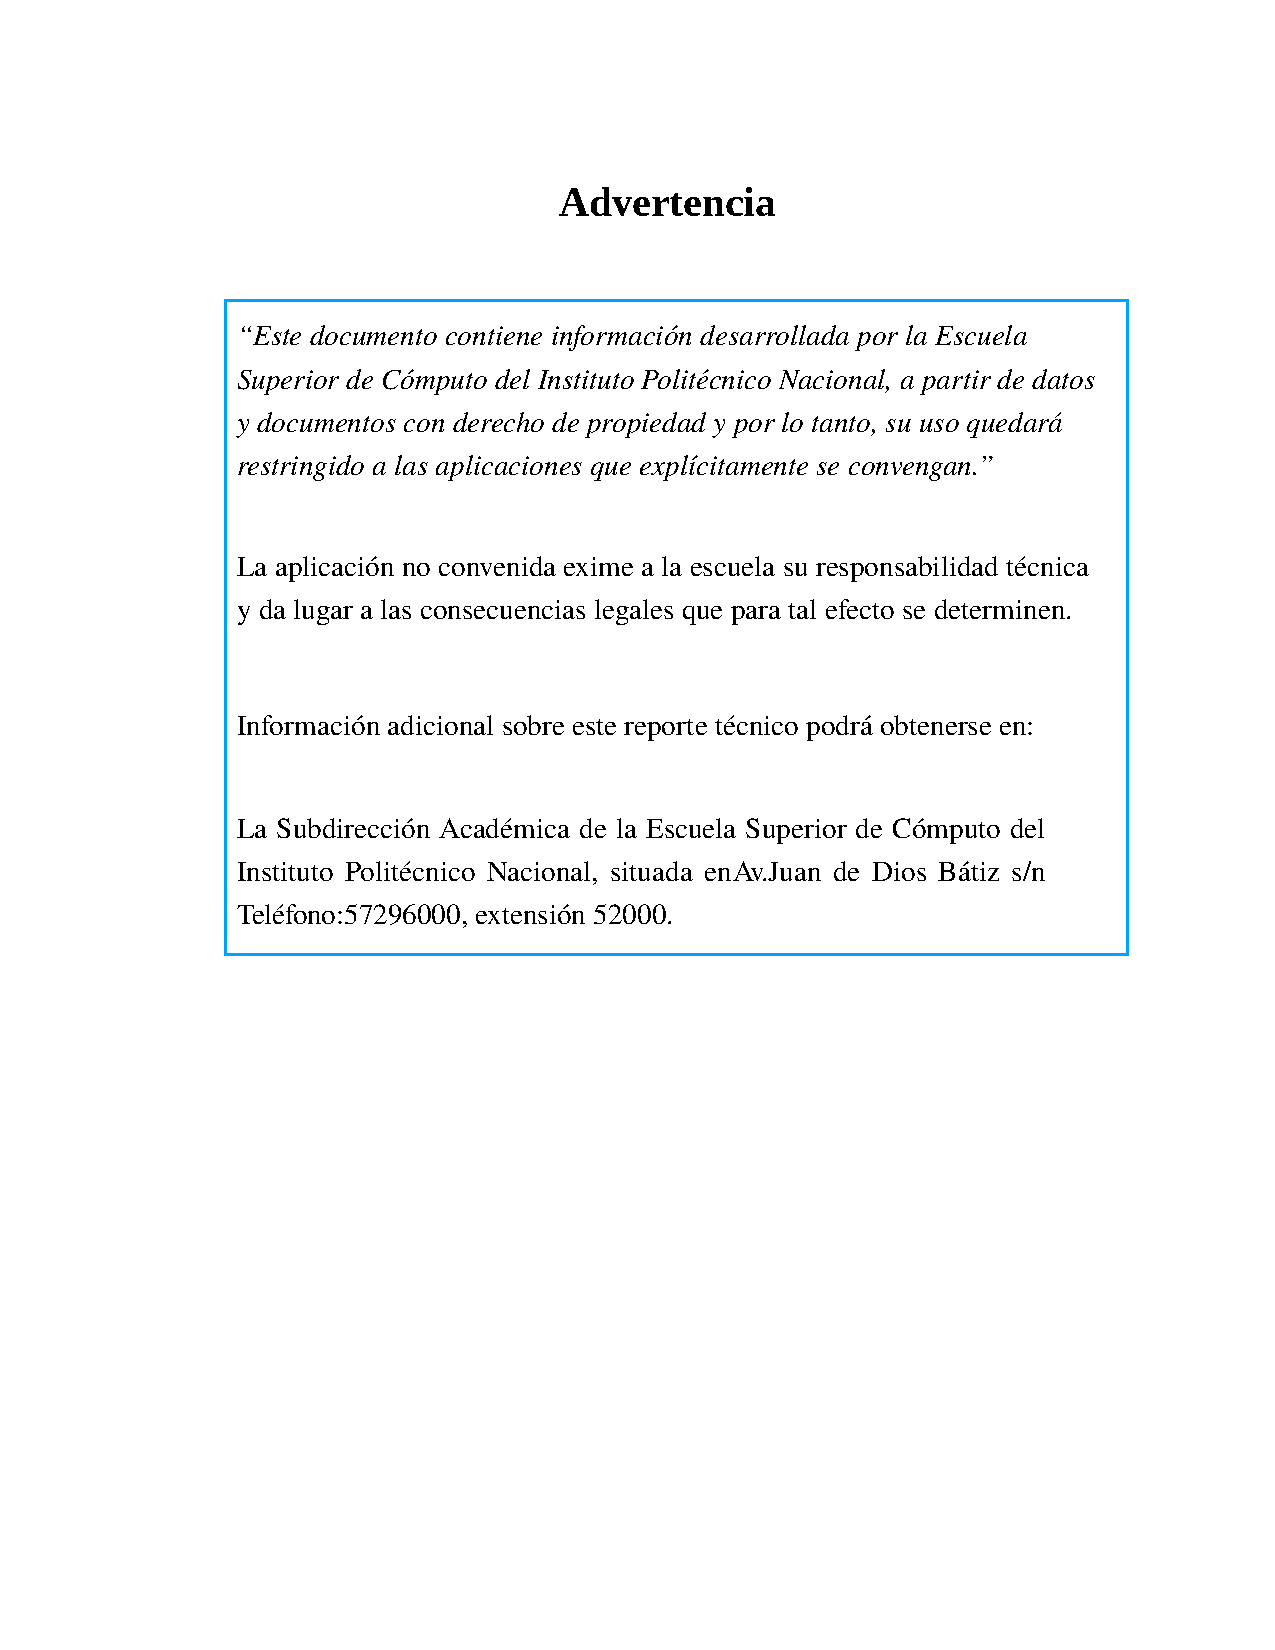
\includepdf[pages=1-1]{Advertencia.pdf}

%\maketitle
 
%=========================================================
% Hoja de revisión
%\makeDocInfo
%\vspace{0.5cm}
%\makeElemRefs
%\makeDocRefs
%\makeObservaciones[3cm]
%\vspace{0.5cm}
%\makeFirmas

%=========================================================
% Indices del documento
\frontmatter
 \LRCornerWallPaper{1}{cdt/theme/pleca.png}
\tableofcontents
\listoffigures
%\listoftables
\mainmatter

% Para esconder la información del documentador se descomenta el \hideControlVersion
 \hideControlVersion
 
%=========================================================
\chapter{Introducción}\label{chp:introduccion}
    \cfinput{Introduccion/introduccion}
    
%=========================================================
\chapter{Análisis y Diseño del Sistema}
	\cfinput{cap2/SistemadeSeguimiento}

%===========================================================
%\chapter{Modelo de Comportamiento del Paciente: Casos de Uso del paciente \label{chp:modeloComportamientoPaciente}}
%%En este capítulo se describen los casos de uso referentes al registro y modificación de la información de las escuelas y del comité asociado a cada una de ellas. \bigskip
%\newpage
%En este capítulo se describen los casos de uso referentes a las acciones que tendrá el rol del Paciente dentro de la aplicación Rem-Pills. \bigskip
%
%\begin{objetivos}[Elementos de un caso de uso]
%	\item {\bf Resumen:} Descripción textual del caso de uso.
%	\item {\bf Actores:} Lista de los actores que intervienen en el caso de uso.
%	\item {\bf Propósito:} Una breve descripción del objetivo que busca el actor al ejecutar el caso de uso.
%	\item {\bf Entradas:} Lista de los datos de entrada requeridos durante la ejecución del caso de uso.
%	\item {\bf Salidas:} Lista de los datos de salida que presenta el sistema durante la ejecución del caso de uso.
%	\item {\bf Precondiciones:} Descripción de las operaciones o condiciones que se deben cumplir previamente para que el caso de uso pueda ejecutarse correctamente.
%	\item {\bf Postcondiciones:} Lista de los cambios que ocurrirán en el sistema después de la ejecución del caso de uso y de las consecuencias en el sistema.
%	\item {\bf Reglas de negocio:} Lista de las reglas que describen, limitan o controlan algún aspecto del negocio del caso de uso.
%	\item {\bf Mensajes:} Lista de los posibles mensajes que pueden surgir durante la ejecución del caso de uso.
%	\item {\bf Trayectorias:} Secuencia de los pasos que ejecutará el caso de uso.
%\end{objetivos}
%
%\cfinput{ModeloPaciente/cup1/uc}
%\cfinput{ModeloPaciente/cup2/uc}
%\cfinput{ModeloPaciente/cup3/uc}
%\cfinput{ModeloPaciente/cup4/uc}
%\cfinput{ModeloPaciente/cup5/uc}
%\cfinput{ModeloPaciente/cup6/uc}
%\cfinput{ModeloPaciente/cup7/uc}
%\cfinput{ModeloPaciente/cup8/uc}
%\cfinput{ModeloPaciente/cup9/uc}
%\cfinput{ModeloPaciente/cup10/uc}
%\cfinput{ModeloPaciente/cup11/uc}
%\cfinput{ModeloPaciente/cup12/uc}
%\cfinput{ModeloPaciente/cup13/uc}
%\cfinput{ModeloPaciente/cup14/uc}
%\cfinput{ModeloPaciente/cup15/uc}
%\cfinput{ModeloPaciente/cup16/uc}
%\cfinput{ModeloPaciente/cup17/uc}
%\cfinput{ModeloPaciente/cup18/uc}
%\cfinput{ModeloPaciente/cup19/uc}
%\cfinput{ModeloPaciente/cup20/uc}
%\cfinput{ModeloPaciente/cup21/uc}
%\cfinput{ModeloPaciente/cup22/uc}
%\cfinput{ModeloPaciente/cup23/uc}
%\cfinput{ModeloPaciente/cup24/uc}
%\cfinput{ModeloPaciente/cup25/uc}
%\cfinput{ModeloPaciente/cup26/uc}
%\cfinput{ModeloPaciente/cup27/uc}
%\newpage
%%%%%%%%%%%%%%%%%%%%%%%%%%%%%%%%%%%%%%%%%%%%%%%%
%\chapter{Modelo de Comportamiento del Doctor: Casos de Uso del doctor \label{chp:modeloComportamientoDoctor}}
%%En este capítulo se describen los casos de uso referentes al registro y modificación de la información de las escuelas y del comité asociado a cada una de ellas. \bigskip
%\newpage
%En este capítulo se describen los casos de uso referentes a las acciones que tendrá el rol del Doctor dentro de la aplicación Rem-Pills. \bigskip
%
%\begin{objetivos}[Elementos de un caso de uso]
%	\item {\bf Resumen:} Descripción textual del caso de uso.
%	\item {\bf Actores:} Lista de los actores que intervienen en el caso de uso.
%	\item {\bf Propósito:} Una breve descripción del objetivo que busca el actor al ejecutar el caso de uso.
%	\item {\bf Entradas:} Lista de los datos de entrada requeridos durante la ejecución del caso de uso.
%	\item {\bf Salidas:} Lista de los datos de salida que presenta el sistema durante la ejecución del caso de uso.
%	\item {\bf Precondiciones:} Descripción de las operaciones o condiciones que se deben cumplir previamente para que el caso de uso pueda ejecutarse correctamente.
%	\item {\bf Postcondiciones:} Lista de los cambios que ocurrirán en el sistema después de la ejecución del caso de uso y de las consecuencias en el sistema.
%	\item {\bf Reglas de negocio:} Lista de las reglas que describen, limitan o controlan algún aspecto del negocio del caso de uso.
%	\item {\bf Mensajes:} Lista de los posibles mensajes que pueden surgir durante la ejecución del caso de uso.
%	\item {\bf Trayectorias:} Secuencia de los pasos que ejecutará el caso de uso.
%\end{objetivos}
%
%\cfinput{ModeloDoctor/cud1/uc}
%\cfinput{ModeloDoctor/cud2/uc}
%\cfinput{ModeloDoctor/cud3/uc}
%\cfinput{ModeloDoctor/cud4/uc}
%\cfinput{ModeloDoctor/cud5/uc}
%\cfinput{ModeloDoctor/cud6/uc}
%\cfinput{ModeloDoctor/cud7/uc}
%\cfinput{ModeloDoctor/cud8/uc}
%\cfinput{ModeloDoctor/cud9/uc}
%\cfinput{ModeloDoctor/cud10/uc}
%\cfinput{ModeloDoctor/cud11/uc}
%\cfinput{ModeloDoctor/cud12/uc}
%\cfinput{ModeloDoctor/cud13/uc}
%\cfinput{ModeloDoctor/cud14/uc}
%\cfinput{ModeloDoctor/cud15/uc}
%
%
%
%%%%%%%%%%%%%%%%%%%%%%%%%%%%%%%%%%%%%%%%%%%%%%%%%%%
%\chapter{Modelo de Comportamiento del Auxiliar: Casos de Uso del auxiliar \label{chp:modeloComportamientoAuxiliar}}
%%En este capítulo se describen los casos de uso referentes al registro y modificación de la información de las escuelas y del comité asociado a cada una de ellas. \bigskip
%\newpage
%En este capítulo se describen los casos de uso referentes a las acciones que tendrá el rol del Auxiliar dentro de la aplicación Rem-Pills. \bigskip
%
%\begin{objetivos}[Elementos de un caso de uso]
%	\item {\bf Resumen:} Descripción textual del caso de uso.
%	\item {\bf Actores:} Lista de los actores que intervienen en el caso de uso.
%	\item {\bf Propósito:} Una breve descripción del objetivo que busca el actor al ejecutar el caso de uso.
%	\item {\bf Entradas:} Lista de los datos de entrada requeridos durante la ejecución del caso de uso.
%	\item {\bf Salidas:} Lista de los datos de salida que presenta el sistema durante la ejecución del caso de uso.
%	\item {\bf Precondiciones:} Descripción de las operaciones o condiciones que se deben cumplir previamente para que el caso de uso pueda ejecutarse correctamente.
%	\item {\bf Postcondiciones:} Lista de los cambios que ocurrirán en el sistema después de la ejecución del caso de uso y de las consecuencias en el sistema.
%	\item {\bf Reglas de negocio:} Lista de las reglas que describen, limitan o controlan algún aspecto del negocio del caso de uso.
%	\item {\bf Mensajes:} Lista de los posibles mensajes que pueden surgir durante la ejecución del caso de uso.
%	\item {\bf Trayectorias:} Secuencia de los pasos que ejecutará el caso de uso.
%\end{objetivos}
%
%\cfinput{ModeloAuxiliar/cua1/uc}
%\cfinput{ModeloAuxiliar/cua2/uc}
%\cfinput{ModeloAuxiliar/cua3/uc}
%\cfinput{ModeloAuxiliar/cua4/uc}
%\cfinput{ModeloAuxiliar/cua5/uc}
%\cfinput{ModeloAuxiliar/cua6/uc}
%\cfinput{ModeloAuxiliar/cua7/uc}
%\cfinput{ModeloAuxiliar/cua8/uc}
%\cfinput{ModeloAuxiliar/cua9/uc}
%\cfinput{ModeloAuxiliar/cua10/uc}
%\cfinput{ModeloAuxiliar/cua11/uc}
%\cfinput{ModeloAuxiliar/cua12/uc}
%\cfinput{ModeloAuxiliar/cua13/uc}
%\cfinput{ModeloAuxiliar/cua14/uc}
%\cfinput{ModeloAuxiliar/cua15/uc}
%
%
%\section{Interfaces del sistema}
%\cfinput{ModeloPaciente/cup1/ui}
%\cfinput{ModeloPaciente/cup2/ui}
%\cfinput{ModeloPaciente/cup3/ui}
%\cfinput{ModeloPaciente/cup4/ui}
%\cfinput{ModeloPaciente/cup5/ui}
%\cfinput{ModeloPaciente/cup6/ui}
%\cfinput{ModeloPaciente/cup7/ui}
%\cfinput{ModeloPaciente/cup8/ui}
%\cfinput{ModeloPaciente/cup9/ui}
%\cfinput{ModeloPaciente/cup10/ui}
%\cfinput{ModeloPaciente/cup11/ui}
%\cfinput{ModeloPaciente/cup12/ui}
%\cfinput{ModeloPaciente/cup13/ui}
%\cfinput{ModeloPaciente/cup14/ui}
%\cfinput{ModeloPaciente/cup15/ui}
%\cfinput{ModeloPaciente/cup16/ui}
%\cfinput{ModeloPaciente/cup17/ui}
%\cfinput{ModeloPaciente/cup18/ui}
%\cfinput{ModeloPaciente/cup19/ui}
%\cfinput{ModeloPaciente/cup20/ui}
%\cfinput{ModeloPaciente/cup21/ui}
%\cfinput{ModeloPaciente/cup22/ui}
%\cfinput{ModeloPaciente/cup23/ui}
%\cfinput{ModeloPaciente/cup24/ui}
%\cfinput{ModeloPaciente/cup25/ui}
%\cfinput{ModeloPaciente/cup26/ui}
%\cfinput{ModeloPaciente/cup27/ui}
%
%\section{Modelo de Interacción}
%
%\cfinput{ModeloInteraccion/mensajes}
%
%\section{Modelo de Negocios}
%
%\cfinput{ModeloNegocios/reglas}
\chapter{Resultados}
\cfinput{Resultados/Resultados}

\chapter{Pruebas}
\cfinput{Pruebas/pruebas}

\chapter{Conclusión}
\cfinput{Conclusion/conclusion}

\chapter{Trabajo a Futuro}
\cfinput{TrabajoaFuturo/TrabajoaFuturo}

%%Referencias
\chapter{Bibliografía}
\cfinput{Referencias/referencias}
%===========================================================

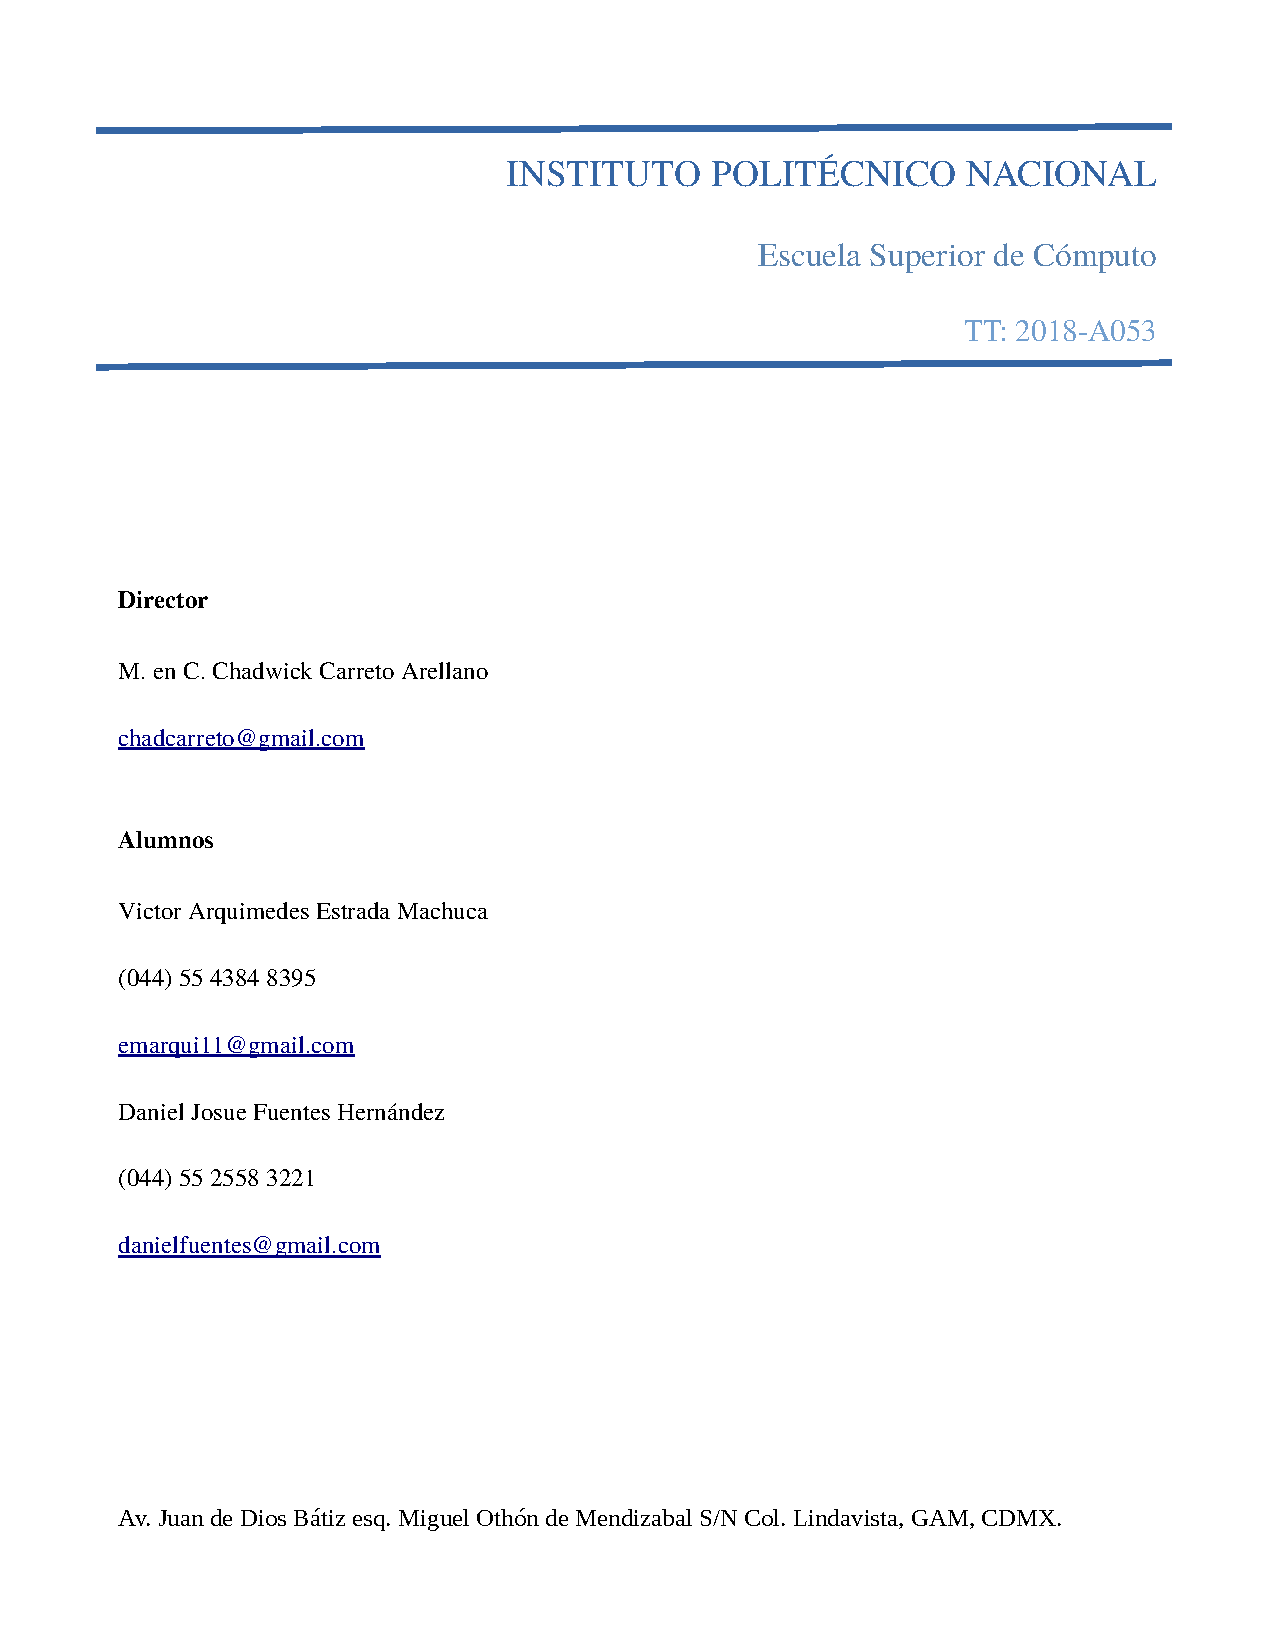
\includepdf[pages=1-1]{contactos.pdf}

   
%=========================================================
%\chapter{Marco Teórico}\label{chp:marcoTeorico}
%    \cfinput{MarcoTeorico/marcoteorico}
    
%=========================================================
%\chapter{Glosario de términos}\label{chp:glosarioTerminos}
%    \cfinput{ModeloNegocios/glosario}
%\chapter{Requerimientos}\label{chp:requerimientos}
%
\subsection{Módulo de Rastreo}

\begin{ReqUser}
	\reqUserItem{RU-MR1}{Rastrear Dispositivo}{La \refStake{Víctima} requiere de un mecanismo que le permita rastrear los puntos de la ciudad por los que su dispositivo ha pasado.}{\media}{\begin{Titemize}
	\Titem \refSistReq{RS-MR1}
    \Titem \refSistReq{RS-MR2}
    \Titem \refSistReq{RS-MR3}
	\end{Titemize}}{\corregir}
    
    \reqUserItem{RU-MR2}{Bloquear Dispositivo}{La \refStake{Víctima} requiere de un mecanismo que evite que el asaltante pueda desbloquear su teléfono.}{\alta}{\refSistReq{RS-MR4}}{\corregir}
\end{ReqUser}

\begin{ReqSist}
	\reqSistItem{RS-MR1}{Activar Dispositivo}{La aplicación debe activarse con la configuración propuesta del usuario si existe, deberá utilizar una configuración por defecto si nunca se ha configurado.}{\alta}{\refUserReq{RU-MR1}}{Funcional}
    
    \reqSistItem{RS-MR2}{Ubicar Dispositivo}{La aplicación deberá conectarse con el servidor de \textbf{Coffee Software} para actualizar su ubicación cada cierto tiempo definido por la \refStake{Víctima} o por la configuración por defecto.}{\media}{\refUserReq{RU-MR1}}{}
    
    \reqSistItem{RS-MR3}{Mostrar la ubicación del dispositivo}{La aplicación web deberá mostrar la ruta que el dispositivo tuvo hasta su última conexión.}{\media}{\refUserReq{RU-MR1}}{}
    
    \reqSistItem{RS-MR4}{Bloquear Dispositivo}{La aplicación móvil deberá bloquear el acceso al dispositivo una vez esta ha sido activada, haciendo parecer que se encuentra apagado.}{\alta}{\refUserReq{RU-MR2}}{}
    
\end{ReqSist}

%=========================================================
%\chapter{Modelo de negocio}\label{chp:modeloNegocios}
%    \cfinput{ModeloNegocios/modelo}
%%    \cfinput{ModeloNegocios/estructura}
%%    \cfinput{ModeloNegocios/registro}
%%    \cfinput{ModeloNegocios/informacion-base}
%%    \cfinput{ModeloNegocios/plan-accion}
%%    \cfinput{ModeloNegocios/seguimiento}
%%    \cfinput{ModeloNegocios/reglas}
%%    \cfinput{ModeloNegocios/indicadores-agua}
%%    \cfinput{ModeloNegocios/indicadores-residuos}
%%    \cfinput{ModeloNegocios/indicadores-energia}
%%    \cfinput{ModeloNegocios/indicadores-biodiversidad}
%%    \cfinput{ModeloNegocios/indicadores-ambienteEscolar}
%%    \cfinput{ModeloNegocios/indicadores-consumoResponsable}
%    
%===========================================================
%\chapter{Modelo de comportamiento}\label{chp:modeloComportamiento}
%  \cfinput{ModeloComportamiento/comportamiento}

%===========================================================
%\chapter{Modelo de comportamiento del módulo: Consulta de Profesores \label{chp:modeloComportamientoProfesores}}
%En este capítulo se describen los casos de uso referentes al registro y modificación de la información de las escuelas y del comité asociado a cada una de ellas. \bigskip
%
%     \begin{objetivos}[Elementos de un caso de uso]
%	\item {\bf Resumen:} Descripción textual del caso de uso.
%	\item {\bf Actores:} Lista de los actores que intervienen en el caso de uso.
%	\item {\bf Propósito:} Una breve descripción del objetivo que busca el actor al ejecutar el caso de uso.
%	\item {\bf Entradas:} Lista de los datos de entrada requeridos durante la ejecución del caso de uso.
%	\item {\bf Salidas:} Lista de los datos de salida que presenta el sistema durante la ejecución del caso de uso.
%	\item {\bf Precondiciones:} Descripción de las operaciones o condiciones que se deben cumplir previamente para que el caso de uso pueda ejecutarse correctamente.
%	\item {\bf Postcondiciones:} Lista de los cambios que ocurrirán en el sistema después de la ejecución del caso de uso y de las consecuencias en el sistema.
%	\item {\bf Reglas de negocio:} Lista de las reglas que describen, limitan o controlan algún aspecto del negocio del caso de uso.
%	\item {\bf Errores:} Lista de los posibles errores que pueden surgir durante la ejecución del caso de uso.
%	\item {\bf Trayectorias:} Secuencia de los pasos que ejecutará el caso de uso.
%    \end{objetivos}

%	\cfinput{ModuloRegistro/cur1/uc}
    	
%\chapter{Modelo de interacción con el usuario}\label{chp:modeloInteraccionUsuario}
%\cfinput{ModeloInteraccion/interaccion}

%---------------------------------------------------------------------
%\section{Interfaces del subsistema: Registro de escuelas}



%---------------------------------------------------------------------

%\section{Diseño de mensajes}
% \cfinput{ModeloInteraccion/mensajes}

%% Referencias
% \bibliographystyle{plain}
% \bibliography{referencias}
%\addcontentsline{toc}{chapter}{Referencias}


\end{document}